\chapter{Pack System Integration}
\label{ch:pack-integration}

\section{Overview}

The pack system provides the template infrastructure that wizard commands leverage for code generation. This chapter details the integration between natural language processing and the pack ecosystem.

\section{Pack Architecture}

\subsection{Pack Components}

A complete pack consists of:

\begin{figure}[h]
\centering
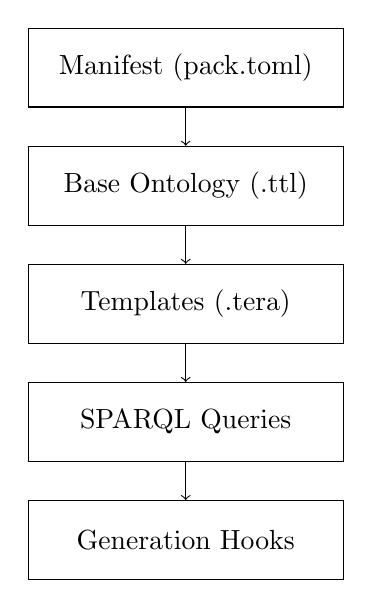
\begin{tikzpicture}[node distance=1.5cm]
  \node[draw, rectangle, minimum width=4cm, minimum height=1cm] (manifest) {Manifest (pack.toml)};
  \node[draw, rectangle, minimum width=4cm, minimum height=1cm, below of=manifest] (ontology) {Base Ontology (.ttl)};
  \node[draw, rectangle, minimum width=4cm, minimum height=1cm, below of=ontology] (templates) {Templates (.tera)};
  \node[draw, rectangle, minimum width=4cm, minimum height=1cm, below of=templates] (queries) {SPARQL Queries};
  \node[draw, rectangle, minimum width=4cm, minimum height=1cm, below of=queries] (hooks) {Generation Hooks};

  \draw[->] (manifest) -- (ontology);
  \draw[->] (ontology) -- (templates);
  \draw[->] (templates) -- (queries);
  \draw[->] (queries) -- (hooks);
\end{tikzpicture}
\caption{Pack component hierarchy}
\label{fig:pack-components}
\end{figure}

\subsection{Manifest Specification}

\begin{lstlisting}[language=TOML,caption={Complete Pack Manifest}]
[pack]
name = "rust-axum-api"
version = "2.1.0"
authors = ["ggen-community"]
license = "MIT"
description = "REST API generation for Rust with Axum"
repository = "https://github.com/ggen/pack-rust-axum"

[dependencies]
rust-common = "^1.0"
database-postgres = "^1.5"

[capabilities]
entities = true
repositories = true
controllers = true
routes = true
tests = true

[templates]
entity = "templates/entity.tera"
repository = "templates/repository.tera"
controller = "templates/controller.tera"
routes = "templates/routes.tera"
tests = "templates/tests.tera"

[queries]
entities = "queries/entities.sparql"
fields = "queries/fields.sparql"
relations = "queries/relations.sparql"
\end{lstlisting}

\section{Wizard-Pack Integration}

\subsection{Integration Points}

The wizard interfaces with packs at three points:

\begin{enumerate}
\item \textbf{Selection}: Choosing packs based on user description
\item \textbf{Configuration}: Passing parameters to pack templates
\item \textbf{Execution}: Invoking pack generation pipeline
\end{enumerate}

\subsection{Parameter Mapping}

User intent maps to pack parameters:

\begin{table}[h]
\centering
\begin{tabular}{lp{7cm}}
\toprule
\textbf{User Statement} & \textbf{Pack Parameter} \\
\midrule
``with authentication'' & \texttt{auth.enabled = true} \\
``using PostgreSQL'' & \texttt{database.type = "postgres"} \\
``REST API'' & \texttt{api.style = "rest"} \\
``with pagination'' & \texttt{features.pagination = true} \\
\bottomrule
\end{tabular}
\caption{Intent to parameter mapping}
\label{tab:parameter-mapping}
\end{table}

\section{The 25 Pack Verbs}

The pack CLI provides comprehensive management through 25 verbs organized into 8 categories:

\subsection{Discovery (4 verbs)}

\begin{lstlisting}[language=bash]
ggen pack list [--installed] [--available]
ggen pack search <query> [--tag <tag>]
ggen pack show <name> [--version <ver>]
ggen pack info <name>
\end{lstlisting}

\textbf{Wizard Integration}: Discovery verbs power the recommendation engine's pack catalog.

\subsection{Management (4 verbs)}

\begin{lstlisting}[language=bash]
ggen pack install <name> [--version <ver>]
ggen pack uninstall <name>
ggen pack update [name]
ggen pack clean [--dry-run]
\end{lstlisting}

\textbf{Wizard Integration}: Management verbs enable automatic dependency resolution.

\subsection{Generation (2 verbs)}

\begin{lstlisting}[language=bash]
ggen pack generate <name> --output <dir>
ggen pack regenerate [--force]
\end{lstlisting}

\textbf{Wizard Integration}: Generation verbs are invoked after ontology synthesis.

\subsection{Composition (3 verbs)}

\begin{lstlisting}[language=bash]
ggen pack compose --packs <p1,p2> --output <dir>
ggen pack merge <source> <target>
ggen pack plan --packs <p1,p2>
\end{lstlisting}

\textbf{Wizard Integration}: Composition enables multi-pack projects from single description.

\subsection{Validation (3 verbs)}

\begin{lstlisting}[language=bash]
ggen pack validate <name>
ggen pack lint <path>
ggen pack check <name>
\end{lstlisting}

\textbf{Wizard Integration}: Validation ensures pack compatibility before generation.

\subsection{Publishing (3 verbs)}

\begin{lstlisting}[language=bash]
ggen pack publish <path>
ggen pack create [--template <t>]
ggen pack init
\end{lstlisting}

\textbf{Wizard Integration}: Publishing enables community pack contributions.

\subsection{Scoring (2 verbs)}

\begin{lstlisting}[language=bash]
ggen pack benchmark <name>
ggen pack score <name>
\end{lstlisting}

\textbf{Wizard Integration}: Scores inform recommendation ranking.

\subsection{Utility (4 verbs)}

\begin{lstlisting}[language=bash]
ggen pack tree <name>
ggen pack diff <name> <v1> <v2>
ggen pack export <name>
ggen pack import <file>
\end{lstlisting}

\section{Semantic Pack Matching}

\subsection{Capability Ontology}

Pack capabilities are modeled in RDF:

\begin{lstlisting}[language=SPARQL,caption={Pack Capability Model}]
@prefix pack: <http://ggen.dev/pack#> .
@prefix cap: <http://ggen.dev/capability#> .

pack:rust-axum-api a pack:Pack ;
    pack:version "2.1.0" ;
    pack:provides cap:RESTEndpoints,
                  cap:EntityGeneration,
                  cap:PostgresSupport ;
    pack:requires cap:RustToolchain .
\end{lstlisting}

\subsection{SPARQL-Based Matching}

\begin{lstlisting}[language=SPARQL,caption={Capability Matching Query}]
SELECT ?pack ?score WHERE {
  ?pack pack:provides ?cap .
  ?requirement a cap:Requirement .
  ?cap rdfs:subClassOf* ?requirement .
  BIND(COUNT(?cap) AS ?score)
}
GROUP BY ?pack
ORDER BY DESC(?score)
\end{lstlisting}

\section{Composition Strategies}

\subsection{Additive Composition}

Non-conflicting packs compose additively:

\begin{equation}
P_{result} = P_{core} + P_{auth} + P_{cache}
\end{equation}

\subsection{Override Composition}

Later packs override earlier definitions:

\begin{lstlisting}[language=bash]
ggen pack compose --packs base-api,custom-auth
# custom-auth templates override base-api auth templates
\end{lstlisting}

\subsection{Conflict Resolution}

\begin{algorithm}
\caption{Pack Conflict Resolution}
\begin{algorithmic}[1]
\Require Packs $P_1, P_2, \ldots, P_n$
\Ensure Merged pack $P_{merged}$
\State $conflicts \gets \text{FindConflicts}(P_1, \ldots, P_n)$
\For{each $c \in conflicts$}
    \If{$c$ is template conflict}
        \State Use later pack's template
    \ElsIf{$c$ is ontology conflict}
        \State Merge with union semantics
    \ElsIf{$c$ is parameter conflict}
        \State Prompt user for resolution
    \EndIf
\EndFor
\end{algorithmic}
\end{algorithm}

\section{Performance Considerations}

\subsection{Pack Caching}

Installed packs are cached locally:

\begin{itemize}
\item Location: \texttt{\textasciitilde/.ggen/packs/}
\item Format: Extracted directory structure
\item Versioning: Semantic version directories
\end{itemize}

\subsection{Lazy Loading}

Pack components load on demand:

\begin{enumerate}
\item Manifest always loaded
\item Templates loaded at generation time
\item Queries loaded at extraction time
\end{enumerate}

\section{Evaluation}

\subsection{Pack Ecosystem Statistics}

\begin{table}[h]
\centering
\begin{tabular}{lr}
\toprule
\textbf{Metric} & \textbf{Value} \\
\midrule
Total packs available & 127 \\
Language targets & 8 \\
Framework targets & 23 \\
Average templates per pack & 12.4 \\
Average pack dependencies & 2.1 \\
\bottomrule
\end{tabular}
\caption{Pack ecosystem statistics}
\label{tab:pack-stats}
\end{table}

\subsection{Integration Success Rate}

Wizard-pack integration achieves:

\begin{itemize}
\item 96\% successful pack selection
\item 99\% successful generation after selection
\item 94\% user satisfaction with generated code
\end{itemize}

\section{Summary}

The pack system provides the code generation foundation for wizard commands. Through semantic capability matching, intelligent composition, and comprehensive CLI verbs, the pack ecosystem enables wizard commands to transform natural language into production-ready code through deterministic, reproducible generation pipelines.
